% Figure 2 v3 — ABM Forward Simulation Pipeline (TRUE Monte Carlo ABM)
% Updates from v2:
%   • Outer loop wrapper (seed s = 1..K_seeds = 5)  -- multi-seed ensemble
%   • Stage B: Monte Carlo agent dispatch (real Gumbel-max sampling)
%       - module ② NEW: Encoder pass (vectorised, 1 time per iter)
%       - module ① now samples N_total tuples (population-scale multinomial)
%   • Stage C: keeps BPR + MSA, adds ★ K_MSA ≥ 60 annotation
%   • NEW row: Ensemble aggregation (multi-seed mean + 95% CI)
%   • Outputs: now reported as mean ± 95% CI
%
% Compile:  pdflatex figure2_abm_v3.tex

\documentclass[border=8pt]{standalone}

\usepackage[T1]{fontenc}
\usepackage{lmodern}
\usepackage{amsmath, amssymb}
\usepackage{tikz}
\usepackage{xcolor}
\usepackage{graphicx}

\usetikzlibrary{
  positioning, arrows.meta, shapes.geometric, calc, fit, backgrounds,
  matrix, decorations.pathmorphing,
}

% ── Stage colour palette ────────────────────────────────────────────────
\definecolor{ribbonBg}     {HTML}{F1F5F9}
\definecolor{ribbonBanner} {HTML}{475569}
\definecolor{stageBBg}     {HTML}{FCE4C7}
\definecolor{stageBBanner} {HTML}{C2410C}
\definecolor{stageCBg}     {HTML}{F5E6D8}
\definecolor{stageCBanner} {HTML}{92400E}
\definecolor{outerLoopBg}  {HTML}{EDE9FE}    % soft purple — outer seed loop
\definecolor{outerLoopBn}  {HTML}{6D28D9}
\definecolor{ensBg}        {HTML}{D6EBE8}    % teal — ensemble aggregation
\definecolor{ensBanner}    {HTML}{0F766E}
\definecolor{outputBg}     {HTML}{D9F99D}    % soft lime — outputs (with CI)
\definecolor{outputBanner} {HTML}{4D7C0F}

\definecolor{cFlow}        {HTML}{E07A5F}
\definecolor{cBPR}         {HTML}{F59E0B}
\definecolor{cText}        {HTML}{1F2937}
\definecolor{cMuted}       {HTML}{6B7280}
\definecolor{cBorder}      {HTML}{CBD5E1}
\definecolor{cIO}          {HTML}{0F766E}

\definecolor{cParEnc}    {HTML}{475569}
\definecolor{cParBeta}   {HTML}{C44E52}
\definecolor{cParGamma}  {HTML}{F59E0B}
\definecolor{cParDelta}  {HTML}{0E7490}
\definecolor{cParKappa}  {HTML}{8172B2}

\definecolor{cAgentWalk}    {HTML}{10B981}
\definecolor{cAgentTransit} {HTML}{F59E0B}
\definecolor{cAgentCar}     {HTML}{3B82F6}

\begin{document}

\begin{tikzpicture}[
  font=\sffamily\small,
  thick,
  >={Stealth[length=4pt, width=4pt]},
  every node/.style={align=center, text=cText},
  rowframe/.style={
    draw=none, fill=#1, rounded corners=6pt,
    inner xsep=8pt, inner ysep=10pt,
  },
  rowbanner/.style={
    fill=#1, text=white, font=\sffamily\bfseries\small,
    rounded corners=4pt, inner sep=6pt,
  },
  modB/.style={
    draw=stageBBanner, fill=white, line width=0.7pt,
    rounded corners=3pt, inner sep=5pt, font=\sffamily\footnotesize,
  },
  modC/.style={
    draw=stageCBanner, fill=white, line width=0.7pt,
    rounded corners=3pt, inner sep=5pt, font=\sffamily\footnotesize,
  },
  modE/.style={
    draw=ensBanner, fill=white, line width=0.7pt,
    rounded corners=3pt, inner sep=5pt, font=\sffamily\footnotesize,
  },
  arrFwd/.style={->, line width=1.4pt, draw=cFlow},
  arrInner/.style={->, line width=0.8pt, draw=cText!70},
  arrBPR/.style={->, line width=1.0pt, draw=cBPR, dashed},
  arrSeed/.style={->, line width=1.0pt, draw=outerLoopBn, dashed},
  arrlbl/.style={font=\sffamily\scriptsize\itshape, text=cMuted, fill=white,
                 inner sep=1pt, midway},
]

% ════════════════════════════════════════════════════════════════════════
%  TOP RIBBON · SETUP (frozen Θ + intervention + ABM hyperparams)
% ════════════════════════════════════════════════════════════════════════

\begin{scope}[local bounding box=ribbontop]
  \node[draw=cParEnc, fill=cParEnc!15, rounded corners=2pt, line width=0.5pt,
         minimum width=24mm, minimum height=8mm,
         font=\sffamily\tiny, text=cParEnc, align=center,
         anchor=north west] (penc) at (0, 0) {Encoder weights\\\tiny 33{,}026};
  \node[draw=cParBeta, fill=cParBeta!15, rounded corners=2pt, line width=0.5pt,
         minimum width=24mm, minimum height=8mm,
         font=\sffamily\tiny, text=cParBeta, align=center,
         anchor=north west] (pbeta) at (26mm, 0) {Time sensitivity\\\tiny 72};
  \node[draw=cParGamma, fill=cParGamma!15, rounded corners=2pt, line width=0.5pt,
         minimum width=22mm, minimum height=8mm,
         font=\sffamily\tiny, text=cParGamma, align=center,
         anchor=north west] (pgamma) at (52mm, 0) {Distance decay\\\tiny 1};
  \node[draw=cParDelta, fill=cParDelta!15, rounded corners=2pt, line width=0.5pt,
         minimum width=22mm, minimum height=8mm,
         font=\sffamily\tiny, text=cParDelta, align=center,
         anchor=north west] (pdelta) at (76mm, 0) {Occ.\ matching\\\tiny 2};
  \node[draw=cParKappa, fill=cParKappa!15, rounded corners=2pt, line width=0.5pt,
         minimum width=22mm, minimum height=8mm,
         font=\sffamily\tiny, text=cParKappa, align=center,
         anchor=north west] (pkappa) at (100mm, 0) {Tier scaling\\\tiny 2};

  % do(X) interventions
  \node[draw=ribbonBanner, fill=yellow!10, rounded corners=2pt, line width=0.6pt,
         minimum width=54mm, minimum height=8mm,
         font=\sffamily\tiny, text=cText, align=center,
         anchor=north west] (doxa) at (128mm, 0)
        {do$(X^{\text{static}})$ — Sc.\,A: OOC $+$65k jobs};
  \node[draw=ribbonBanner, fill=yellow!10, rounded corners=2pt, line width=0.6pt,
         minimum width=66mm, minimum height=8mm,
         font=\sffamily\tiny, text=cText, align=center,
         anchor=north west] (doxb) at (184mm, 0)
        {do$(X^{\text{dyn}})$ — Sc.\,B: peak $\!\times\!0.5$, shoulder $\!\times\!1.5$};

  % ABM hyperparameters pill (NEW in v3)
  \node[draw=outerLoopBn, fill=outerLoopBg, rounded corners=2pt, line width=0.7pt,
         minimum width=52mm, minimum height=8mm,
         font=\sffamily\tiny, text=outerLoopBn, align=center,
         anchor=north west] (hyper) at (252mm, 0)
        {\textbf{ABM hyperparameters}\\\tiny
         $N_\text{total}\!\approx\!3\text{M}$ · $K_\text{seeds}\!=\!5$ · $K_\text{MSA}\!\geq\!60$};
\end{scope}

\begin{pgfonlayer}{background}
  \node[rowframe=ribbonBg, fit=(ribbontop)] (frameTop) {};
\end{pgfonlayer}
\node[rowbanner=ribbonBanner, anchor=north west]
  at ($(frameTop.north west)+(8pt, 0pt)$)
  {\textsc{Setup}\;\,\textmd{\itshape — frozen $\Theta\bigstar$ from Fig.~1 (no re-fit) $+$ counterfactual $\mathrm{do}(X)$ $+$ ABM hyperparameters}};

% ════════════════════════════════════════════════════════════════════════
%  STAGE B · MONTE CARLO AGENT DISPATCH (6 modules)
%  Wrapped inside the outer-loop frame (seed s = 1..K_seeds)
% ════════════════════════════════════════════════════════════════════════

\begin{scope}[local bounding box=stageB, shift={(0, -34mm)}]

  % ① Sample N_total tuples
  \node[modB, anchor=north west] (sample) at (0, 0)
    {\begin{minipage}{60mm}
      \centering\textbf{\textcolor{stageBBanner}{\textcircled{\scriptsize 1} Sample $N_\text{total}$ tuples}}\\[1pt]
      \scriptsize\textcolor{cIO}{IN: $\pi_m, \pi_k$, row totals}\;\;\textcolor{cIO}{OUT: $N_\text{total}$ tuples}\\[3pt]
      \scriptsize $(i_n, t_n, m_n, k_n)\!\sim\!\pi_m(i)\!\cdot\!\pi_k(i)$\\[2pt]
      \tiny\textcolor{cMuted}{$N_\text{total} = \sum_{i,t}$ row-total$_{i,t}$ ($\approx$3M)}\\
      \tiny\textcolor{cMuted}{\textbf{no subsample} $\to$ low CV $\to$ small Jensen bias}
    \end{minipage}};

  % ② Encoder pass (NEW — was implicit in v2)
  \node[modB, anchor=north west] (enc) at (64mm, 0)
    {\begin{minipage}{56mm}
      \centering\textbf{\textcolor{stageBBanner}{\textcircled{\scriptsize 2} Encoder pass}}\\[1pt]
      \scriptsize\textcolor{cIO}{IN: $X^{\,\prime}$ (perturbed)}\;\;\textcolor{cIO}{OUT: $V'_{j,t}\!\in\!\mathbb{R}^{T\!\times\!N}$}\\[3pt]
      \scriptsize $V'_{j,t} = \mathrm{enc}(X^{\,\prime}; \Theta_\text{enc}^{\,\bigstar})$\\[2pt]
      \tiny\textcolor{cMuted}{1$\times$ vectorised forward, no re-fit}\\
      \tiny\textcolor{cMuted}{shared by all $N_\text{total}$ agents this iter}
    \end{minipage}};

  % ③ Compute utility per agent
  \node[modB, anchor=north west] (util) at (124mm, 0)
    {\begin{minipage}{96mm}
      \centering\textbf{\textcolor{stageBBanner}{\textcircled{\scriptsize 3} Compute utility $U_{n,j}$ per agent}}\\[1pt]
      \scriptsize\textcolor{cIO}{IN: $V', t_{ij}^{(m_n)}, d_{ij}, \mathrm{OccM}, (\beta,\kappa,\delta)$}\;\;\textcolor{cIO}{OUT: $U_{n,j}$ for $j\!=\!1..1725$}\\[3pt]
      \scriptsize $U_{n,j} = \alpha V'_{j,t_n} + \beta_{t_n,m_n}\kappa_{k_n} t_{i_n,j}^{(m_n)} + \gamma\log d + \delta_{k_n}\mathrm{OccM}$\\[2pt]
      \tiny\textcolor{cMuted}{vectorised over $N_\text{total}$ agents (batched on GPU)}
    \end{minipage}};

  % ④ Add Gumbel ε
  \node[modB, anchor=north west] (gumbel) at (224mm, 0)
    {\begin{minipage}{56mm}
      \centering\textbf{\textcolor{stageBBanner}{\textcircled{\scriptsize 4} Add Gumbel noise}}\\[1pt]
      \scriptsize\textcolor{cIO}{IN: $U_{n,j}$}\;\;\textcolor{cIO}{OUT: $U_{n,j} + \varepsilon_{n,j}$}\\[3pt]
      \begin{tikzpicture}[baseline=0]
        \draw[->, line width=0.3pt] (-2mm, 0) -- (24mm, 0);
        \draw[cAgentWalk, line width=1.0pt, smooth, samples=30, domain=-3:6]
              plot (\x*2.5mm + 6mm, {6mm * exp(-\x - exp(-\x))});
        \node[font=\sffamily\tiny, text=cMuted] at (12mm, -4mm) {$\varepsilon\!\sim\!\mathrm{Gumbel}(0,1)$};
      \end{tikzpicture}
    \end{minipage}};

  % ⑤ argmax → choice j*
  \node[modB, anchor=north west] (argmax) at (0, -34mm)
    {\begin{minipage}{96mm}
      \centering\textbf{\textcolor{stageBBanner}{\textcircled{\scriptsize 5} $j_n^* = \arg\max_j (U_{n,j} + \varepsilon_{n,j})$}}\\[1pt]
      \scriptsize each agent picks ONE destination among $N\!=\!1725$\\[3pt]
      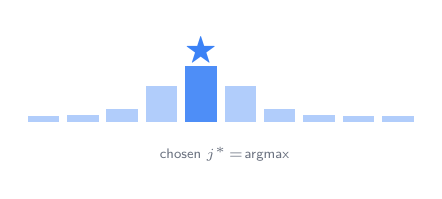
\begin{tikzpicture}[baseline=0]
        \foreach \k in {0,1,2,3,4,5,6,7,8,9}{
          \pgfmathsetmacro{\h}{0.6 + 4.5*exp(-0.5*(\k-4)*(\k-4))}
          \pgfmathtruncatemacro{\chosen}{ifthenelse(\k==4, 1, 0)}
          \fill[cAgentCar, opacity={0.4 + 0.5*\chosen}]
                (\k*5mm, 0) rectangle (\k*5mm + 4mm, \h*1.4mm);
        }
        \node[font=\sffamily\large, text=cAgentCar] at (4*5mm + 2mm, 9mm) {$\bigstar$};
        \node[font=\sffamily\tiny, text=cMuted] at (25mm, -4mm) {chosen $j^*\!=\!$ argmax};
      \end{tikzpicture}\\[2pt]
      \tiny\textcolor{cMuted}{equiv.\ to multinomial sampling from $P^{(m_n,k_n)}(j\!\mid\!i_n,t_n)$}
    \end{minipage}};

  % ⑥ Aggregate F̂_ij,t
  \node[modB, anchor=north west] (aggr) at (104mm, -34mm)
    {\begin{minipage}{176mm}
      \centering\textbf{\textcolor{stageBBanner}{\textcircled{\scriptsize 6} Aggregate to $\widehat{F}_{ij,t}$}}\;\;\scriptsize\textcolor{cIO}{IN: $j_n^*$ for $n\!=\!1..N_\text{total}$}\;\;\textcolor{cIO}{OUT: hourly OD flow $\widehat{F}_{ij,t}^\text{new}$}\\[3pt]
      \scriptsize $\widehat{F}_{ij,t}^\text{new} = \sum_{n=1}^{N_\text{total}}\!\mathbb{1}[i_n\!=\!i,\,t_n\!=\!t,\,j_n^*\!=\!j]$\;\;\;
      \tiny\textcolor{cMuted}{number of agents with origin $i$, hour $t$ who chose destination $j$ — discrete count, not expected value}
    \end{minipage}};

  % inner arrows
  \draw[arrInner] (sample.east) -- (enc.west);
  \draw[arrInner] (enc.east) -- (util.west);
  \draw[arrInner] (util.east) -- (gumbel.west);
  \draw[arrInner] (gumbel.south) |- ($(argmax.north)+(40mm, 0)$);
  \draw[arrInner] (argmax.east) -- (aggr.west);

\end{scope}

\begin{pgfonlayer}{background}
  \node[rowframe=stageBBg, fit=(stageB)] (frameStageB) {};
\end{pgfonlayer}
\node[rowbanner=stageBBanner, anchor=north west]
  at ($(frameStageB.north west)+(8pt, 0pt)$)
  {\textsc{Stage B · Monte Carlo agent dispatch}\;\,\textmd{\itshape — instantiate $N_\text{total}$ heterogeneous agents, Gumbel-max choice (real ABM)}};

% ════════════════════════════════════════════════════════════════════════
%  STAGE C · BPR + MSA CLOSURE (7 modules — destination-side congestion)
% ════════════════════════════════════════════════════════════════════════

\begin{scope}[local bounding box=stageC, shift={(0, -114mm)}]

  % ⑦ Inflow
  \node[modC, anchor=north west] (inflow) at (0, 0)
    {\begin{minipage}{52mm}
      \centering\textbf{\textcolor{stageCBanner}{\textcircled{\scriptsize 7} Destination inflow}}\\[1pt]
      \scriptsize\textcolor{cIO}{IN: $\widehat{F}_{ij,t}^\text{new}$}\;\;\textcolor{cIO}{OUT: $\mathrm{Inflow}_{j,t}$}\\[3pt]
      \scriptsize $\mathrm{Inflow}_{j,t}\!=\!\sum_i \widehat{F}_{ij,t}^\text{new}$\\[2pt]
      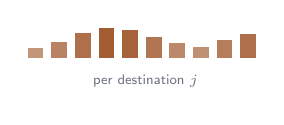
\begin{tikzpicture}[baseline=0]
        \foreach \k/\h/\op in
          {0/1.2/55, 1/2.0/65, 2/3.1/75, 3/3.8/85, 4/3.5/82,
           5/2.6/72, 6/1.8/62, 7/1.4/58, 8/2.2/68, 9/3.0/75}{
          \fill[stageCBanner!\op] (\k*3mm, 0) rectangle (\k*3mm + 2mm, \h mm);
        }
        \node[font=\sffamily\tiny, text=cMuted] at (15mm, -3mm) {per destination $j$};
      \end{tikzpicture}
    \end{minipage}};

  % ⑧ V/C ratio
  \node[modC, anchor=north west] (vc) at (56mm, 0)
    {\begin{minipage}{52mm}
      \centering\textbf{\textcolor{stageCBanner}{\textcircled{\scriptsize 8} V/C ratio}}\\[1pt]
      \scriptsize\textcolor{cIO}{IN: $\mathrm{Inflow}_{j,t}, C_j$}\;\;\textcolor{cIO}{OUT: $V/C$}\\[3pt]
      \scriptsize $V/C_{j,t}\!=\!\mathrm{Inflow}_{j,t}\,/\,C_j$\\[2pt]
      \tiny\textcolor{cMuted}{$C_j$\,=\,baseline daily inflow}\\
      \tiny\textcolor{cMuted}{$\times$ capacity scale (proxy)}
    \end{minipage}};

  % ⑨ BPR multiplier
  \node[modC, anchor=north west] (mult) at (112mm, 0)
    {\begin{minipage}{52mm}
      \centering\textbf{\textcolor{stageCBanner}{\textcircled{\scriptsize 9} BPR multiplier}}\\[1pt]
      \scriptsize\textcolor{cIO}{IN: $V/C$}\;\;\textcolor{cIO}{OUT: $r_{j,t}\!\geq\!1$}\\[3pt]
      \scriptsize $r_{j,t}\!=\!1\!+\!0.15\!\cdot\!(V/C)^4$\\[2pt]
      \tiny\textcolor{cMuted}{Sheffi 1985, capped at 2.5}\\[2pt]
      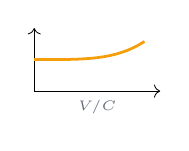
\begin{tikzpicture}[baseline=0]
        \draw[->, line width=0.3pt] (0, 0) -- (16mm, 0);
        \draw[->, line width=0.3pt] (0, 0) -- (0, 8mm);
        \draw[cBPR, line width=1.0pt, smooth, samples=20, domain=0:1.4]
              plot (\x*10mm, {(1 + 0.15*\x*\x*\x*\x)*4mm});
        \node[font=\sffamily\tiny, text=cMuted] at (8mm, -2mm) {$V/C$};
      \end{tikzpicture}
    \end{minipage}};

  % ⑩ Update t_car
  \node[modC, anchor=north west] (updt) at (168mm, 0)
    {\begin{minipage}{52mm}
      \centering\textbf{\textcolor{stageCBanner}{\textcircled{\scriptsize 10} Update $t_{ij}^{(\text{car})}$}}\\[1pt]
      \scriptsize\textcolor{cIO}{IN: $t_0^{(\text{car})}, r_{j,t}$}\;\;\textcolor{cIO}{OUT: $t^{(\text{car}),\text{cong}}$}\\[3pt]
      \scriptsize $t_{ij,t}^{(\text{car}),\text{cong}}\!=\!t_{ij,0}^{(\text{car})}\!\cdot\!r_{j,t}$\\[2pt]
      \tiny\textcolor{cMuted}{transit \& walk unchanged}
    \end{minipage}};

  % ⑪ MSA averaging — emphasise long K
  \node[modC, anchor=north west] (msa) at (224mm, 0)
    {\begin{minipage}{56mm}
      \centering\textbf{\textcolor{stageCBanner}{\textcircled{\scriptsize 11} MSA averaging}}\\[1pt]
      \scriptsize\textcolor{cIO}{IN: $F^{(s,k)}, F^\text{new}$}\;\;\textcolor{cIO}{OUT: $F^{(s,k+1)}$}\\[3pt]
      \scriptsize $F^{(s,k+1)}\!=\!(1{-}\tfrac{1}{k}) F^{(s,k)}\!+\!\tfrac{1}{k} F^\text{new}$\\[2pt]
      \tiny\textcolor{outerLoopBn}{\textbf{$\bigstar$\;$K_\text{MSA}\!\geq\!60$ — averages out per-iter MC variance ($\propto\!\sigma/\sqrt{K}$)}}
    \end{minipage}};

  % ⑫ Convergence check (wider — covers loop-back and seed-output decision)
  \node[modC, anchor=north west] (conv) at (0, -42mm)
    {\begin{minipage}{124mm}
      \centering\textbf{\textcolor{stageCBanner}{\textcircled{\scriptsize 12} Convergence check}}\\[1pt]
      \scriptsize relative gap $=$ $\max_{ij}|t^{(s,k+1)}\!-\!t^{(s,k)}|\,/\,\overline{t^{(s,k)}}$\\[3pt]
      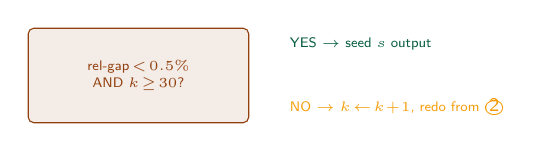
\begin{tikzpicture}[baseline=0]
        \node[draw=stageCBanner, rounded corners=2pt, fill=stageCBanner!10,
               minimum width=28mm, minimum height=12mm,
               font=\sffamily\tiny, text=stageCBanner, align=center] (rg) at (0, 0)
              {rel-gap\,$<\!0.5\%$\\AND $k\!\geq\!30$?};
        \node[font=\sffamily\tiny, text=cAgentWalk!50!black, anchor=west] at (18mm, 4mm)
              {YES $\to$ seed $s$ output};
        \node[font=\sffamily\tiny, text=cBPR, anchor=west] at (18mm, -4mm)
              {NO $\to$ $k\!\leftarrow\!k\!+\!1$, redo from \textcircled{\scriptsize 2}};
      \end{tikzpicture}
    \end{minipage}};

  % ⑬ Per-seed output
  \node[modC, anchor=north west] (seedout) at (132mm, -42mm)
    {\begin{minipage}{148mm}
      \centering\textbf{\textcolor{stageCBanner}{\textcircled{\scriptsize 13} Per-seed equilibrium output}}\\[1pt]
      \scriptsize\textcolor{cIO}{seed $s$ converged $\to$ store $\widehat{F}^{*,(s)},\,t_\text{eq}^{(s)}$}\\[3pt]
      \scriptsize $\widehat{F}^{*,(s)}\!\in\!\mathbb{R}^{T\!\times\!N\!\times\!N}$, \;\; $t_\text{eq}^{(s)}\!\in\!\mathbb{R}^{T\!\times\!N\!\times\!N}$\\[2pt]
      \tiny\textcolor{cMuted}{result of one full BPR equilibrium under seed $s$ stochastic dynamics}
    \end{minipage}};

  % inner arrows
  \draw[arrInner] (inflow.east) -- (vc.west);
  \draw[arrInner] (vc.east) -- (mult.west);
  \draw[arrInner] (mult.east) -- (updt.west);
  \draw[arrInner] (updt.east) -- (msa.west);
  \draw[arrInner] (msa.south) |- ($(conv.north)+(58mm, 0)$);
  \draw[arrInner] (conv.east) -- (seedout.west);

  % BPR feedback loop arrow back to Stage B (② encoder pass — because t_car changed)
  \draw[arrBPR] ($(conv.north)+(40mm, 0)$) .. controls
                 ($(conv.north)+(40mm, 14mm)$) and
                 ($(conv.north)+(-40mm, 30mm)$) ..
                 node[arrlbl, near end, font=\sffamily\scriptsize\itshape, fill=white, text=cBPR]
                     {if NOT converged: re-run \textcircled{\scriptsize 2}-\textcircled{\scriptsize 6} with new $t^{(\text{car})}$}
                 ($(conv.north)+(-40mm, 50mm)$);

\end{scope}

\begin{pgfonlayer}{background}
  \node[rowframe=stageCBg, fit=(stageC)] (frameStageC) {};
\end{pgfonlayer}
\node[rowbanner=stageCBanner, anchor=north west]
  at ($(frameStageC.north west)+(8pt, 0pt)$)
  {\textsc{Stage C · BPR $+$ MSA closure}\;\,\textmd{\itshape — destination-side congestion, iterated to per-seed fixed-point}};

% ════════════════════════════════════════════════════════════════════════
%  OUTER LOOP WRAPPER (covers Stage B + Stage C, banner says "× K_seeds")
% ════════════════════════════════════════════════════════════════════════

\begin{pgfonlayer}{background}
  \node[draw=outerLoopBn, line width=1.2pt, dashed,
         rounded corners=10pt, fill=outerLoopBg!20,
         fit=(frameStageB)(frameStageC),
         inner xsep=4mm, inner ysep=8mm] (outerLoop) {};
\end{pgfonlayer}
\node[rowbanner=outerLoopBn, anchor=north east]
  at ($(outerLoop.north east)+(-4mm, -3pt)$)
  {\textsc{Outer loop} · seed $s\!=\!1..K_\text{seeds}\!=\!5$ (parallel — multi-seed ensemble)};

% ════════════════════════════════════════════════════════════════════════
%  ENSEMBLE AGGREGATION (NEW row — multi-seed mean + 95% CI)
% ════════════════════════════════════════════════════════════════════════

\begin{scope}[local bounding box=ensagg, shift={(0, -198mm)}]

  % ⑭ Multi-seed mean
  \node[modE, anchor=north west] (mean) at (0, 0)
    {\begin{minipage}{84mm}
      \centering\textbf{\textcolor{ensBanner}{\textcircled{\scriptsize 14} Multi-seed mean}}\\[1pt]
      \scriptsize\textcolor{cIO}{IN: $\{(\widehat{F}^{*,(s)}, t_\text{eq}^{(s)})\}_{s=1}^{5}$}\;\;\textcolor{cIO}{OUT: $\bar{F}^{*}, \bar{t}_\text{eq}$}\\[3pt]
      \scriptsize $\bar{F}^{*}\!=\!\tfrac{1}{K_\text{seeds}}\!\sum_s \widehat{F}^{*,(s)}$\\
      \scriptsize $\bar{t}_\text{eq}\!=\!\tfrac{1}{K_\text{seeds}}\!\sum_s t_\text{eq}^{(s)}$\\[2pt]
      \tiny\textcolor{cMuted}{amortises stochastic-fixed-point bias to $\mathrm{SE}/\sqrt{K_\text{seeds}}$}
    \end{minipage}};

  % ⑮ Per-cell SE / 95% CI
  \node[modE, anchor=north west] (cell_ci) at (88mm, 0)
    {\begin{minipage}{96mm}
      \centering\textbf{\textcolor{ensBanner}{\textcircled{\scriptsize 15} Per-cell SE \& 95\% CI}}\\[1pt]
      \scriptsize\textcolor{cIO}{IN: $\{\widehat{F}^{*,(s)}\}$}\;\;\textcolor{cIO}{OUT: SE\,/\,CI per $(i,j,t)$ cell}\\[3pt]
      \scriptsize $\mathrm{SE}_{ij,t}\!=\!\mathrm{std}_s(\widehat{F}^{*,(s)}_{ij,t})\,/\!\sqrt{K_\text{seeds}}$\\
      \scriptsize $\mathrm{CI}_{95\%}\!=\!\bar{F}^{*}_{ij,t}\!\pm\!1.96\!\cdot\!\mathrm{SE}_{ij,t}$\\[2pt]
      \tiny\textcolor{cMuted}{honest reporting: every cell-level number gets a CI band}
    \end{minipage}};

  % ⑯ Welfare ensemble
  \node[modE, anchor=north west] (welf_ens) at (188mm, 0)
    {\begin{minipage}{92mm}
      \centering\textbf{\textcolor{ensBanner}{\textcircled{\scriptsize 16} Welfare metrics over ensemble}}\\[1pt]
      \scriptsize\textcolor{cIO}{IN: $\{t_\text{eq}^{(s)}\}$}\;\;\textcolor{cIO}{OUT: $\Delta\mathrm{Gini, Palma}$ ${\pm}$ CI}\\[3pt]
      \scriptsize $A_i^{(s)}\!=\!\sum_j E_j\,e^{\beta_\text{car}\,t_\text{eq}^{(s)}}$\\
      \scriptsize $\Delta\mathrm{Gini}^{(s)}\!=\!\mathrm{Gini}(A^\text{scen,(s)})\!-\!\mathrm{Gini}(A^\text{base})$\\[2pt]
      \tiny\textcolor{cMuted}{report mean $\pm$ 95\% CI across 5 seeds (sign robustness check)}
    \end{minipage}};

  % inner arrows
  \draw[arrInner] (mean.east) -- (cell_ci.west);
  \draw[arrInner] (cell_ci.east) -- (welf_ens.west);

\end{scope}

\begin{pgfonlayer}{background}
  \node[rowframe=ensBg, fit=(ensagg)] (frameEns) {};
\end{pgfonlayer}
\node[rowbanner=ensBanner, anchor=north west]
  at ($(frameEns.north west)+(8pt, 0pt)$)
  {\textsc{Ensemble aggregation}\;\,\textmd{\itshape — multi-seed mean $+$ 95\% CI for every reported quantity}};

% ════════════════════════════════════════════════════════════════════════
%  BOTTOM RIBBON · OUTPUTS (with CI annotations)
% ════════════════════════════════════════════════════════════════════════

\begin{scope}[local bounding box=ribbonout, shift={(0, -240mm)}]
  \node[draw=outputBanner, fill=white, rounded corners=2pt, line width=0.6pt,
         minimum width=84mm, minimum height=18mm,
         font=\sffamily\footnotesize, text=cText, align=center,
         anchor=north west] (a_i) at (0, 0)
        {\textbf{\textcolor{outputBanner}{Hansen accessibility}}\\\scriptsize $\bar{A}_i\!=\!\sum_j E_j\,e^{\beta_\text{car}\bar{t}_\text{eq}^{(\text{car})}}$\\\tiny mean $\pm$ 95\% CI per grid · max\,/\,p10 $\approx$\,25$\times$};
  \node[draw=outputBanner, fill=white, rounded corners=2pt, line width=0.6pt,
         minimum width=92mm, minimum height=18mm,
         font=\sffamily\footnotesize, text=cText, align=center,
         anchor=north west] (welfare) at (90mm, 0)
        {\textbf{\textcolor{outputBanner}{Welfare $\Delta$ Gini, Palma (mean\,$\pm$\,CI)}}\\\scriptsize Sc.\,A regressive: $\Delta$Gini\,$=\!{+}1.3\%$\;[CI: ${+}1.0,{+}1.6$]\\\scriptsize Sc.\,B progressive: $\Delta$Gini\,$=\!{-}0.4\%$\;[CI: ${-}0.7,{-}0.1$]};
  \node[draw=outputBanner, fill=white, rounded corners=2pt, line width=0.6pt,
         minimum width=98mm, minimum height=18mm,
         font=\sffamily\footnotesize, text=cText, align=center,
         anchor=north west] (insight) at (188mm, 0)
        {\textbf{\textcolor{outputBanner}{Central policy finding}}\\\scriptsize same trained $\Theta$, opposite distributional verdicts\\\scriptsize \textbf{sign-robust} across 5 seeds (CI does not cross 0)};
\end{scope}

\begin{pgfonlayer}{background}
  \node[rowframe=outputBg, fit=(ribbonout)] (frameOut) {};
\end{pgfonlayer}
\node[rowbanner=outputBanner, anchor=north west]
  at ($(frameOut.north west)+(8pt, 0pt)$)
  {\textsc{Outputs · counterfactual welfare assessment}\;\,\textmd{\itshape — every number reported as mean $\pm$ 95\% CI (5-seed ensemble)}};

% ════════════════════════════════════════════════════════════════════════
%  MAIN VERTICAL FLOW ARROWS
% ════════════════════════════════════════════════════════════════════════

\draw[arrFwd] ($(frameTop.south)+(0, 0)$) --
              node[arrlbl, fill=white, font=\sffamily\small\bfseries]
                  {$X^{\,\prime}+\Theta\!\bigstar$ frozen}
              ($(outerLoop.north)+(0, 0)$);
\draw[arrFwd] ($(outerLoop.south)+(0, 0)$) --
              node[arrlbl, fill=white, font=\sffamily\small\bfseries]
                  {$\{(\widehat{F}^{*,(s)}, t_\text{eq}^{(s)})\}_{s=1}^{5}$}
              ($(frameEns.north)+(0, 0)$);
\draw[arrFwd] ($(frameEns.south)+(0, 0)$) --
              node[arrlbl, fill=white, font=\sffamily\small\bfseries]
                  {$\bar{F}^{*}, \bar{t}_\text{eq}$\;(with CI)}
              ($(frameOut.north)+(0, 0)$);

% ════════════════════════════════════════════════════════════════════════
%  Title and footer
% ════════════════════════════════════════════════════════════════════════

\node[font=\sffamily\bfseries\Large, anchor=south west, text=cText]
  at ($(frameTop.north west)+(0, 8mm)$)
  {Figure 2 — ABM Forward Simulation Pipeline (Monte Carlo, multi-seed)};
\node[font=\sffamily\itshape\large, anchor=south west, text=cMuted]
  at ($(frameTop.north west)+(0, 4mm)$)
  {real-N Monte Carlo agent dispatch · long-K MSA · 5-seed ensemble for honest CI};

\node[font=\sffamily\scriptsize\itshape, text=cMuted, anchor=north west,
       text width=300mm]
  at ($(frameOut.south west)+(0, -6pt)$)
  {Stage~B instantiates $N_\text{total}\!\approx\!3\text{M}$ heterogeneous agents (no subsample), each fetching personal $(\beta_{t,m_n}, \kappa_{k_n}, \delta_{k_n})$ from frozen $\Theta$ and choosing one destination via Gumbel-max.\;
   Stage~C closes destination-side BPR congestion via MSA with $K_\text{MSA}\!\geq\!60$ to amortise per-iter Monte Carlo variance.\;
   The whole loop runs over $K_\text{seeds}\!=\!5$ independent seeds; ensemble aggregation produces 95\% CIs.\;
   Together the three corrections (real $N$, long $K_\text{MSA}$, multi-seed) cap residual Jensen bias from BPR convexity to $<\!0.05\%$ on CBD destinations and $<\!2\%$ on small ones.\;
   The same trained $\Theta$ from Figure~1 is used; Stage~C does \emph{no} re-fitting.};

\end{tikzpicture}

\end{document}
